%%
%
%
% ---------------------------------------------------------
% ---- SECTION
% ---------------------------------------------------------
\section{Discretization}
\label{sec-discretization}

In this section, we describe the problem in discrete form ...

% ---------------------------------------------------------
% -- SUBSECTION
% ---------------------------------------------------------
\subsection{Spatial discretization}

% ---------------------------------------------------------
% PARAGRAPH
% ---------------------------------------------------------
\paragraph{Faces and skeleton of the mesh}

The boundary $\dCell{}$ of each element is decomposed in faces, such
that a face $F$ is a subset of $\bodyLag$, and either there are two
cells $\cell_F$ and $\cell_F'$ such that $F = \dCell_F \cap \dCell_F'$
($F$ is then an interior face), or there is a single cell $\cell_F$ such
that $F = \dCell_F \cap \partial \Omega$ ($F$ is then an exterior face).
Let $\dHybridMesh(\bodyLag) = \{ F_i \subset \bodyLag \ \vert \ 1 \leq i
\leq N_{F} \}$ the skeleton of the mesh, collecting all element faces
$F_i$ in the mesh, where $N_{F}$ denotes the number of faces. The set of
faces subjected to Neumann boundary conditions is denoted
$\dHybridMesh{}_{N}^e(\bodyLag)$, and $\dHybridMesh{}_{D}^e(\bodyLag)$
denotes that subjected to Dirichlet boundary conditions. Moreover, let
$\mathcal{F}^i(\bodyLag)$ the set of interior faces. For any cell
$\cell$, let $\mathcal{F}(\cell) = \{ F \in \dHybridMesh \ \vert \ F
\subset \dCell \}$ the set of faces composing the boundary of $\cell$,
and let $N_{\dCell}$ the number of faces in $\dCell$.

% ---------------------------------------------------------
% PARAGRAPH
% ---------------------------------------------------------
\paragraph{Mesh description}

Likewise, one defines the collection of all cells in the mesh
as $\HybridMesh(\bodyLag) = \{ \matI \subset \bodyLag \ \vert \ 1 \leq i
\leq N_{\cell} \}$, where $N_T$ denotes the total number of cells. The
composition of both $\mathcal{T}(\bodyLag)$ and
$\dHybridMesh{}(\bodyLag)$ forms the hybrid mesh
$\HybridMeshWhole({\bodyLag}) = \{ \mathcal{T}(\bodyLag),
\mathcal{F}(\bodyLag) \}$.

% ---------------------------------------------------------
% -- SUBSECTION
% ---------------------------------------------------------
\subsection{Functional discretization}

% ---------------------------------------------------------
% PARAGRAPH
% ---------------------------------------------------------
\paragraph{Discrete functional space}

For a cell $\cell$, we denote $\discreteDisplacementSpaceCell$ an
approximation space of finite dimension for the displacement in the
cell, and $V^h(F)$ that on a face $F \in \mathcal{F}(\cell)$. The
approximation space on $\dCell$ is $V^h(\dCell) = \prod_{F \in
  \mathcal{F}(\cell)} V^h(F)$. Similarly, let $\discreteGradSpaceCell$
the approximation space of the reconstructed gradient and
$\discreteStressSpaceCell$ that chosen for the stress.

\paragraph{Approximation bases. Local unknowns}

Let $\mathfrak{B}_T^h$ denote a basis of dimension $N_T^h$ in
$\discreteDisplacementSpaceCell$, and $\mathfrak{B}_F^h$ a basis of
dimension $N_F^h$ in $V^h(F)$. The specific choice of monomial bases for
$\mathfrak{B}_T^h$ and $\mathfrak{B}_F^h$ is discussed in depth in
\ref{sec_implementation}, though other bases can be chosen.

A function $\tensori{u}{}_{T}^h \in U^h(T)$ (respectively
$\tensori{u}{}_{F}^h \in V^h(F)$), is associated with vector of
coefficients $\mathfrak{U}_T$ of size $N_T^h$ (respectively
$\mathfrak{U}_F$ of size $N_F^h$).

\paragraph{Global Unknowns}

Let $(\tensori{u}{}_{\mathcal{T}}^h, \tensori{u}{}_{\mathcal{F}}^h)
\in U^h(\mathcal{T}) \times U^h(\mathcal{F})$ the global displacement
unknown of problem \eqref{eq_final_problem} in discrete form, where
$\tensori{u}{}_{\mathcal{T}}^h$ and $\tensori{u}{}_{\mathcal{F}}^h$ are
the piece-wise continuous displacements such that:
\begin{equation}
  \begin{aligned}
    \tensori{u}{}_{\mathcal{T}}^h
    \vert_{\cell} = \tensori{u}{}_{\cell}^h = \mathfrak{U}_T \cdot
    \mathfrak{B}_T^h && \forall \cell \in \mathcal{T} && \text{and} &&
    \tensori{u}{}_{\mathcal{F}}^h \vert_{F} = \tensori{u}{}_{F}^h =
    \mathfrak{U}_F \cdot \mathfrak{B}_F^h && \forall F \in \mathcal{F}
  \end{aligned}
\end{equation}
with $U^h(\mathcal{T}) = \prod_{T \in \mathcal{T}} U^h(T)$ and
$U^h(\mathcal{F}) = \prod_{F \in \mathcal{F}} U^h(F)$.

Likewise, let $\tensori{u}{}_{\dCell}^h \in V^h(\dCell)$ such
that $\tensori{u}{}_{\dCell}^h \vert_F = \tensori{u}{}_{F}^h, \forall F
\in \mathcal{F}(\partial T)$, where $V^h(\dCell) = \prod_{F \in
  \mathcal{F}(T)} U^h(F)$. In the following, let
$\mathfrak{U}_{\mathcal{T}}$ the unknown coefficient vector associated
to $\tensori{u}{}^h_{\mathcal{T}}$, $\mathfrak{U}_{\mathcal{F}}$ that to
$\tensori{u}{}^h_{\mathcal{F}}$, and $\mathfrak{U}_{\mathcal{\dCell}}$
that to $\tensori{u}{}^h_{\dCell}$.

% ---------------------------------------------------------
% -- SUBSECTION
% ---------------------------------------------------------
\subsection{Local and global discrete problems}

% ---------------------------------------------------------
% PARAGRAPH
% ---------------------------------------------------------
\subsubsection{Local residual}

In a functional space of finite dimension, the restriction of a linear
form can be represented a vector in the dual space. Hence, let
$\mathfrak{R}_{\cell}$ and $\mathfrak{R}_{\dCell}$ the residual vectors
associated with the the variations of the total
Lagrangian~\eqref{eq_0015}:
\begin{subequations}
  \label{eq_final_problem_00}
  \begin{alignat}{3}
    \mathfrak{R}_{\cell}(\mathfrak{U}_{\cell},
    \mathfrak{U}_{\dCell}) \cdot \mathfrak{\hat{U}}_{T}
    % \int_{\mathcal{T}} R_{\mathcal{T}}(\tensori{u}{}_{\mathcal{T}}, \tensori{u}{}_{\mathcal{F}}) \cdot \tensori{\hat{u}}{}_{\mathcal{T}}
 = & \int_{\cell} \tensorii{P}{}_{\cell}^h : \nabla
    \tensori{\hat{u}}{}_{\cell}^h - \int_{\cell} \tensori{f}{}_V \cdot
    \tensori{\hat{u}}{}_{\cell} - \int_{\dCell{}}
    \tensori{\theta}{}_{\cell}^h \cdot \tensori{\hat{u}}{}_{\cell}^h
    \vert_{\dCell} && \ \ \ \ \ \ \ \ && \forall
    \hat{\mathfrak{U}}_{\cell} % \in \virtualDisplacementSpaceCell
    \label{eq_final_problem_00:eq0} \\
    \mathfrak{R}_{\dCell}(\mathfrak{U}_{\cell},
    \mathfrak{U}_{\dCell}) \cdot \mathfrak{\hat{U}}_{\dCell}
    % \int_{\mathcal{F}} R_{\mathcal{F}}(\tensori{u}{}_{\mathcal{T}}, \tensori{u}{}_{\mathcal{F}}) \cdot \tensori{\hat{u}}{}_{\mathcal{F}}
 = & \int_{\dCell} (\tensori{\theta}{}_{\cell}^h -
    \tensori{t}{}_{\neumannCell}) \cdot \tensori{\hat{u}}{}_{\dCell}^h
    && \ \ \ \ \ \ \ \ && \forall \hat{\mathfrak{U}}_{\dCell}
    % \in \virtualDisplacementSpaceDCell \label{eq_final_problem_00:eq1}
    \label{eq_final_problem_00:eq1} \\
  \end{alignat}
\end{subequations}
where the discrete stress tensor $\tensorii{P}{}_{\cell}^h$ and the
discrete reconstructed gradient
$\tensorii{G}{}_{\cell}^h(\tensori{v}{}_{\cell}^h,
\tensori{v}{}_{\dCell}^h)$ are defined by the discrete forms of
equations \eqref{eq_stress} and \eqref{eq_grad} respectively such that:
\begin{equation}
  \label{eq_stress_discrete}
  \begin{aligned}
    \tensorii{P}{}_{\cell}^h =
    \frac{\partial \mecPotential_{\bodyLag}}{\partial
      \tensorii{G}{}_{\cell}^h} && \text{and} && \int_{\cell}
    \tensorii{G}{}_{\cell}^h : \tensorii{\tau}{}_{\cell}^h =
    \int_{\cell} \nabla \tensori{v}{}_{\cell}^h :
    \tensorii{\tau}{}_{\cell}^h + \int_{\dCell}
    (\tensori{v}{}_{\dCell}^h - \tensori{v}{}_{\cell}^h \vert_{\dCell})
    \cdot \tensorii{\tau}{}_{\cell}^h \vert_{\dCell} \cdot \tensori{n}{}
    && \forall \tensorii{\tau}{}_{\cell}^h \in S^h(\cell)
  \end{aligned}
\end{equation}
and the discrete reconstructed traction $\tensori{\theta}{}_{\cell}^h
= \tensorii{P}{}_{\cell}^h \cdot \tensori{n} + \beta / h_{\cell}
\tensori{J}^h(\tensori{v}{}_{\cell}^h, \tensori{v}{}_{\dCell}^h)$.

The solution of the discrete problem $(\mathfrak{U}_{\cell},
\mathfrak{U}_{\dCell})$ is defined by the fact that the associated
residuals $\mathfrak{R}_{\cell}$ and $\mathfrak{R}_{\dCell}$ must be
zero:
\begin{equation}
  \label{eq_final_problem_000}
  \begin{aligned}
    \mathfrak{R}_{\cell}(\mathfrak{U}_{\cell}, \mathfrak{U}_{\dCell})
    = 0 && \text{and} &&
    \mathfrak{R}_{\dCell}(\mathfrak{U}_{\cell}, \mathfrak{U}_{\dCell})
     = 0
  \end{aligned}
\end{equation}

In practice, the computation of $\mathfrak{R}_{\cell}$ and
$\mathfrak{R}_{\dCell}$ is discussed in depth in \ref{sec_implementation}.

% ---------------------------------------------------------
% PARAGRAPH
% ---------------------------------------------------------
\subsubsection{Global residuals and face assembly}

At the global scale, the solutions
$(\mathfrak{U}_{\mathcal{T}}, \mathfrak{U}_{\mathcal{F}})$ of the
discrete problem satisfies:
\begin{equation}
  \label{eq_final_global_problem_0}
  \begin{aligned}
    \forall \cell \in \mathcal{T}(\bodyLag), \forall
    \hat{\mathfrak{U}}_{\cell},
    \mathfrak{R}_{\cell}(\mathfrak{U}_{\cell}, \mathfrak{U}_{\dCell})
    \cdot \mathfrak{\hat{U}}_{T} & = 0 && \text{and} && \forall
    \hat{\mathfrak{U}}_{\mathcal{F}},
    \mathfrak{R}_{\mathcal{F}}(\mathfrak{U}_{\mathcal{T}},
    \mathfrak{U}_{\mathcal{F}}) \cdot \mathfrak{\hat{U}}_{\mathcal{F}} =
    0
  \end{aligned}
\end{equation}
where the vector
$\mathfrak{R}_{\mathcal{F}}(\mathfrak{U}_{\mathcal{T}},
\mathfrak{U}_{\mathcal{F}})$ is the skeleton residual such that~:
\begin{equation}
  \label{eq_final_problem_0}
  \begin{aligned}
    \mathfrak{R}_{\mathcal{F}}(\mathfrak{U}_{\mathcal{T}},
    \mathfrak{U}_{\mathcal{F}}) \cdot \mathfrak{\hat{U}}_{\mathcal{F}}
    % \int_{\mathcal{F}} R_{\mathcal{F}}(\tensori{u}{}_{\mathcal{T}}, \tensori{u}{}_{\mathcal{F}}) \cdot \tensori{\hat{u}}{}_{\mathcal{F}}
 = & \sum_{F \in \mathcal{F}^i(\bodyLag{})} \int_{F}
    (\tensori{\theta}{}_{\cell_F}^h + \tensori{\theta}{}_{\cell_F '}^h)
    \cdot \tensori{\hat{u}}{}_{F}^h + \sum_{F \in
      \mathcal{F}^e_N(\bodyLag{})} \int_{F}
    (\tensori{\theta}{}_{\cell_F}^h - \neumannLag) \cdot
    \tensori{\hat{u}}{}_{F}^h && \forall
    \hat{\mathfrak{U}}_{\mathcal{F}}
  \end{aligned}
\end{equation}

An interior face $F$ is linked to two adjacent cells $T$ and $T'$, and
each of these cells applies to the other a surface load $\pm
\tensori{t}{}_{T\cap T'}$ through $F$, which is identified with
$\tensori{t}{}_{\neumannCell\cap F}$ in \eqref{eq_final_problem_00:eq1}.
By summation over each face of the structure, these equal contributions
cancel out, which yields the expression of the first argument in the
right-hand side in \eqref{eq_final_problem_0}.

Since exterior faces subjected to Neumann boundary conditions are
linked to a single cell only, $\tensori{t}{}_{\neumannCell} =
\neumannLag$ on $\neumannBoundaryLag{}$, which yields the expression of
the second argument in the right-hand side in
\eqref{eq_final_problem_00:eq1}.

% ---------------------------------------------------------
% -- SUBSECTION
% ---------------------------------------------------------
\subsection{Cell unknowns elimination}

As the cell number of unknowns grows rapidly with the polynomial order
as compared to that in the face (See \ref{sec_shape_functions}), cell
unknowns must be eliminated for the for the method to be numerically
attractive.

In this section, two elimination strategies are examinated. The first
one, presented as the \textit{Cell equilibrium} strategy, has, to our
knowledge, never been introduced in the literature, and arises from the
previous total Lagrangian formulation of HDG methods. The second one
consists in performing a static condensation operation
\cite{abbas_hybrid_2018, abbas_hybrid_2019,di_pietro_hybrid_2015}
following linearization of the problem.

% ---------------------------------------------------------
% PARAGRAPH
% ---------------------------------------------------------
\subsubsection{Cell equilibrium}

This first algorithm considers that the cell displacement unknown
$\mathfrak{U}_{T}$ are defined as implicit functions of the boundary
displacement unknown $\mathfrak{U}_{\dCell}$ as follows:
\begin{equation}
  \label{eq_cell_equilibrium_1}
  \begin{aligned}
    \mathfrak{R}_{T}(\mathfrak{U}_{T}(\mathfrak{U}_{\dCell}),
    \mathfrak{U}_{\dCell}) = 0
  \end{aligned}
\end{equation}
In practice, Nonlinear Equation~\eqref{eq_cell_equilibrium_1} can be
solved by an iterative method. At the global scale, the face residual
can thus be expressed as function of the face displacement, and
satisfies:
\begin{equation}
  \label{eq_cell_equilibrium_face_residual}
  \mathfrak{R}_{\mathcal{F}}(\mathfrak{U}_{\mathcal{T}}\paren{\mathfrak{U}_{\mathcal{F}}},
 \mathfrak{U}_{\mathcal{F}})=0
\end{equation}

Nonlinear Equation~\eqref{eq_cell_equilibrium_face_residual} is
generally solved using an iterative method. For the sake of simplicity,
the Newton method is considered here. Let
\(\iter{n}{\mathfrak{U}_{\mathcal{F}}}\) be the current estimate of the
solution. The correction \(\iter{n}{\delta}\mathfrak{U}_{\mathcal{F}}\)
of this estimate is given by:
\[
\iter{n}{\delta}\mathfrak{U}_{\mathcal{F}}=
-\left( \frac{d\mathfrak{R}_{\mathcal{F}}}{d \mathfrak{U}_{\mathcal{F}}}
\right)^{-1} \,\cdot\,\iter{n}{\mathfrak{R}}_{\mathcal{F}}
\]
with
\(\iter{n}{\delta}\mathfrak{U}_{\mathcal{F}}=\iter{n+1}{\mathfrak{U}_{\mathcal{F}}}-\iter{n}{\mathfrak{U}_{\mathcal{F}}}\).


The jacobian matrix \(\frac{d\mathfrak{R}_{\mathcal{F}}}{d
  \mathfrak{U}_{\mathcal{F}}}\) can be determined using the chain rule,
as follows:
\begin{equation}
  \label{eq_cell_equilibrium_0}
  \begin{aligned}
    % R_{\mathcal{T}}(\mathfrak{U}_{\mathcal{T}})
    % \frac{d \mathfrak{R}_{\mathcal{F}}}{d \mathfrak{U}_{\mathcal{F}}}
    \frac{d\mathfrak{R}_{\mathcal{F}}}{d
      \mathfrak{U}_{\mathcal{F}}}
    = \frac{\partial
      \mathfrak{R}_{\mathcal{F}}}{\partial \mathfrak{U}_{\mathcal{T}}}
    \frac{\partial \mathfrak{U}_{\mathcal{T}}}{\partial
      \mathfrak{U}_{\mathcal{F}}} \cdot \delta
    \mathfrak{U}_{\mathcal{F}} + \frac{\partial
      \mathfrak{R}_{\mathcal{F}}}{\partial \mathfrak{U}_{\mathcal{F}}}
    \cdot \delta \mathfrak{U}_{\mathcal{F}}
  \end{aligned}
\end{equation}
Applying the implicit function theorem to
\eqref{eq_cell_equilibrium_1} yields:
\begin{equation}
  \label{eq_cell_equilibrium_2}
  \begin{aligned}
    \frac{\partial
      \mathfrak{U}_{\mathcal{T}}}{\partial \mathfrak{U}_{\mathcal{F}}} =
    - \frac{\partial \mathfrak{U}_{\mathcal{T}}}{\partial
      \mathfrak{R}_{\mathcal{T}}} \frac{\partial
      \mathfrak{R}_{\mathcal{T}}}{\partial \mathfrak{U}_{\mathcal{F}}}
  \end{aligned}
\end{equation}
Injecting \eqref{eq_cell_equilibrium_2} in
\eqref{eq_cell_equilibrium_0} yields the expression of the derivative of
the face resiudal with respect to the face displacement
\begin{equation}
  \label{eq_cell_equilibrium_3}
  \begin{aligned}
    % \frac{d \mathfrak{R}_{\mathcal{F}}}{d \mathfrak{U}_{\mathcal{F}}}
    \frac{d\mathfrak{R}_{\mathcal{F}}}{d
      \mathfrak{U}_{\mathcal{F}}} = \frac{\partial
      \mathfrak{R}_{\mathcal{T}}}{\partial \mathfrak{U}_{\mathcal{F}}}
    \cdot \delta \mathfrak{U}_{\mathcal{F}} - \frac{\partial
      \mathfrak{R}_{\mathcal{T}}}{\partial \mathfrak{U}_{\mathcal{T}}}
    \frac{\partial \mathfrak{U}_{\mathcal{T}}}{\partial
      \mathfrak{R}_{\mathcal{T}}} \frac{\partial
      \mathfrak{R}_{\mathcal{T}}}{\partial \mathfrak{U}_{\mathcal{F}}}
    \cdot \delta \mathfrak{U}_{\mathcal{F}}
  \end{aligned}
\end{equation}

% ---------------------------------------------------------
% PARAGRAPH
% ---------------------------------------------------------
\subsubsection{Static condensation}

In this section, $\mathfrak{U}_{\mathcal{T}}$ and
$\mathfrak{U}_{\mathcal{F}}$ are assumed to be independent variables.
Again, a Newton method is considered.

At the cell level, the correction of the cell unknown
$\iter{n}{\delta}\mathfrak{U}_{\cell}$ and face unknowns
$\iter{n}{\delta}\mathfrak{U}_{\dCell}$ are given by:
\begin{equation}
\label{eq_static_condensation_final}
\mathcal{K}\,\cdot\,
\begin{pmatrix}
  \iter{n}{\delta}\mathfrak{U}_{\cell}
  \\
  \iter{n}{\delta}\mathfrak{U}_{\dCell}
\end{pmatrix}
= -
\begin{pmatrix}
  \iter{n}{\mathfrak{R}}_{\mathcal{\cell}}
  \\
  \iter{n}{\mathfrak{R}}_{\mathcal{\dCell}}
\end{pmatrix}
\quad\text{with}\quad \mathcal{K} =
\begin{pmatrix}
  \derivtot{\mathfrak{R}_{\cell}}{\mathfrak{U}_{\cell}}
  & \derivtot{\mathfrak{R}_{\cell}}{\mathfrak{U}_{\dCell}} \\
  \derivtot{\mathfrak{R}_{\dCell}}{\mathfrak{U}_{\cell}}
  & \derivtot{\mathfrak{R}_{\dCell}}{\mathfrak{U}_{\dCell}} \\
\end{pmatrix}
=
\begin{pmatrix}
  \mathcal{K}_{\cell\cell} &
  \mathcal{K}_{\cell\dCell} \\
  \mathcal{K}_{\dCell\cell} &
  \mathcal{K}_{\dCell\dCell} \\
\end{pmatrix}
\end{equation}
where the blocks \(\mathcal{K}_{\cell\cell}\),
\(\mathcal{K}_{\cell\dCell}\), \(\mathcal{K}_{\dCell\cell}\) and
\(\mathcal{K}_{\dCell\dCell}\) have been introduced for convenience.

The correction of the cell unknown
$\iter{n}{\delta}\mathfrak{U}_{\cell}$ can thus be expressed as:
\begin{equation}
  \label{eq:cell_unknown_correction}
  \iter{n}{\delta}\mathfrak{U}_{\cell}=
  -\mathcal{K}_{\cell\cell}^{-1}\,\cdot\,\,\iter{n}{\mathfrak{R}}_{\mathcal{\cell}}
  -\mathcal{K}_{\cell\cell}^{-1}\,\cdot\,\mathcal{K}_{\cell\dCell}\,\cdot\,\iter{n}{\delta}\mathfrak{U}_{\dCell}
\end{equation}

The correction of the face unknown
$\iter{n}{\delta}\mathfrak{U}_{\dCell}$ satisfies:
\[
\paren{ \mathcal{K}_{\dCell\dCell}\,
  -\mathcal{K}_{\dCell\cell}\,\cdot\,\mathcal{K}_{\cell\cell}^{-1}\,\cdot\,\mathcal{K}_{\cell\dCell}
 }\,\cdot\, \iter{n}{\delta}\mathfrak{U}_{\dCell}=
-\iter{n}{\mathfrak{R}}_{\mathcal{\dCell}}
+\mathcal{K}_{\dCell\cell}\,\cdot\,\mathcal{K}_{\cell\cell}^{-1}\,\cdot\,\,\iter{n}{\mathfrak{R}}_{\mathcal{\cell}}
\]
or, introducing the condensed quantities
\(\iter{n}{\left.\mathfrak{R}^{c}_{\mathcal{\dCell}}\right.}\) and
\(\mathcal{K}_{\dCell\cell}^{c}\):
\[
\mathcal{K}_{\dCell\dCell}^{c}\,\cdot\,\iter{n}{\delta}\mathfrak{U}_{\dCell}=
-\iter{n}{\left.\mathfrak{R}^{c}_{\mathcal{\dCell}}\right.}
\]

The element contributions
\(\iter{n}{\left.\mathfrak{R}^{c}_{\mathcal{\dCell}}\right.}\) and
\(\mathcal{K}_{\dCell\cell}^{c}\) are then assembled to form the linear
system giving \(\iter{n}{\delta}\mathfrak{U}_{\mathcal{F}}\). Once,
\(\iter{n}{\delta}\mathfrak{U}_{\dCell}\) is known, a decondensation
step is performed to computed \(\iter{n}{\delta}\mathfrak{U}_{\cell}\)
using Equation~\ref{eq:cell_unknown_correction}.


\subsection{Extension to non linear materials with internal state variables}
\label{sec:discretization:extension_to_non_linear_materials}

This section is devoted to the extension of the method to non linear
materials with local internal state variables. Let \(\vec{Y}\) be the
set of internal state variables describing the material. Each cell is
assumed to describe a unique material.

To simplify the presentation and preseve a variational framework, the
behaviour of the material is assumed to be standard
generalized~\cite{moreau_sur_1970,halphen_sur_1975}. The evolution of
the material can thus be described by an incremental lagrangian
\(L_{\cell}^{HDG}\) defined as
follows~\cite{lorentz_variational_1999,forest_localization_2004}:
\begin{equation}
  L_{\cell}^{HDG} = \displaystyle \int_{\cell} \left[
  \mecPotential{}_{\bodyLag{}}+\Delta\,t\,\dissipationPotential\paren{\Frac{\vec{Y}^{\star}-\bts{\vec{Y}}}{\Delta\,t}}
 \right] + \int_{\dCell} \frac{\beta}{2 h_{\cell}} \lVert
  \tensori{J}(\tensori{u}{}_{\cell{}}, \tensori{u}{}_{\dCell{}})
  \rVert^2 - \int_{\cell} \loadLag{} \cdot \tensori{u}{}_{\cell{}} -
  \int_{\neumannCell{}} \neumannCellLoad{} \cdot
  \tensori{u}{}_{\dCell{}}
\end{equation}
where:
\begin{itemize}
  \item \(\dissipationPotential\) denotes the dissipation
  potential.
  \item \(\Delta\,t\) denotes the time increment.
  \item \(\bts{\vec{Y}}\) denotes the value of the internal state
  variables at the beginning of the time step.
\end{itemize}

At this stage, two strategies can be set-up to eliminate the internal
state variables:
\begin{enumerate}
  \item Classically, state variables are assumed to be defined at
  the integration points (or, expressed differently, to be approximated
  in \(L^{2}\)). This strategy is the one used by most finite element
  solvers. In pratice, given the increment of the reconstructed
  gradient, the constitutive equations, expressed as a system of
  ordinary differential equations, are integrated to compute the new
  value of the stress and the consistent tangent operator. This
  strategy, already used by Abbas et
  al.~\cite{abbas_hybrid_2018,abbas_hybrid_2019}, is used in the
  numerical examples of this paper.
  \item The state variables can also be approximated in some
  discrete space on the cell. In this case, the cell resolution
  algorithm could be extended to define the cell displacements and the
  state variables as implicit functions of the face displacements. This
  approach seems \emph{a priori} interesting in at least two cases:
  \begin{itemize}
    \item Applied to plasticity, this approach lead to a en
    potentially efficient multi-field
    plasticity~\cite{simo_computational_1998} method with a low
    computational cost as the extra degrees of freedoms (associated with
    the plastic strains) can be eliminated at the cell level.
    % Static condensation in the context of multi-field plasticty \cite{schroder_static_2015}.
    \item Applied to phase-field damage problems, the
    irreversibility constraint could be treated at the element level by
    defining appropriate Lagrange multiplier that can be eliminated. A
    similar idea was developped by Cicuttin et al. for the elliptic
    obstacle problem~\cite{cicuttin_hybrid_2020}.
  \end{itemize}
  Exploring those two lines of research is left for future
  works.
\end{enumerate}

%Moreover, it allows to consider extending the present cell correction
%iterative resolution to \textit{e.g.} constrained resolution algorithm,
%in order to solve inequality constrained problems, as encountered in
%multi-field plasticity~\cite{schroder_small_2015} for instance.

\subsubsection{Comparison between both schemes}
\label{par_cell_eq}

\paragraph{Static condensation}

The static condensation algorithm is the one used in the literature
\cite{di_pietro_discontinuous-skeletal_2015,cockburn_algorithm_2019,abbas_hybrid_2019-1,abbas_hybrid_2018}
to eliminate cell unknowns. Contrary to the introduced cell resolution
algorithm, this scheme needs not iterate at the cell level to accomodate
the cell correction. The actualization of the cell unknown displacement
by its correction requires that the quantities $\partial
\tensori{u}{}_{\cell}^l / \partial R_{\cell}^{\cell}$ and $\partial
R_{\cell}^{\cell} / \partial \tensori{u}{}_{\dCell}^k$ computed at the
previous iteration are known. From a numerical standpoint, this results
in keeping stiffness matrices blocks (see
Section~\ref{sec_implementation2}) in memory from an iteration to the
other.

\paragraph{Cell equilibrium}

The novel cell resolution scheme needs iterate at the cell level. It
may require to integrate the constitutive equation more times than the
static condensation algorithm does (See
paragraph~\ref{sec:discretization:extension_to_non_linear_materials}).
However, it allows to exactly evaluate the equilibrium of the cell with
its boundary, what does not the former.

\begin{figure}[H]
    \centering
    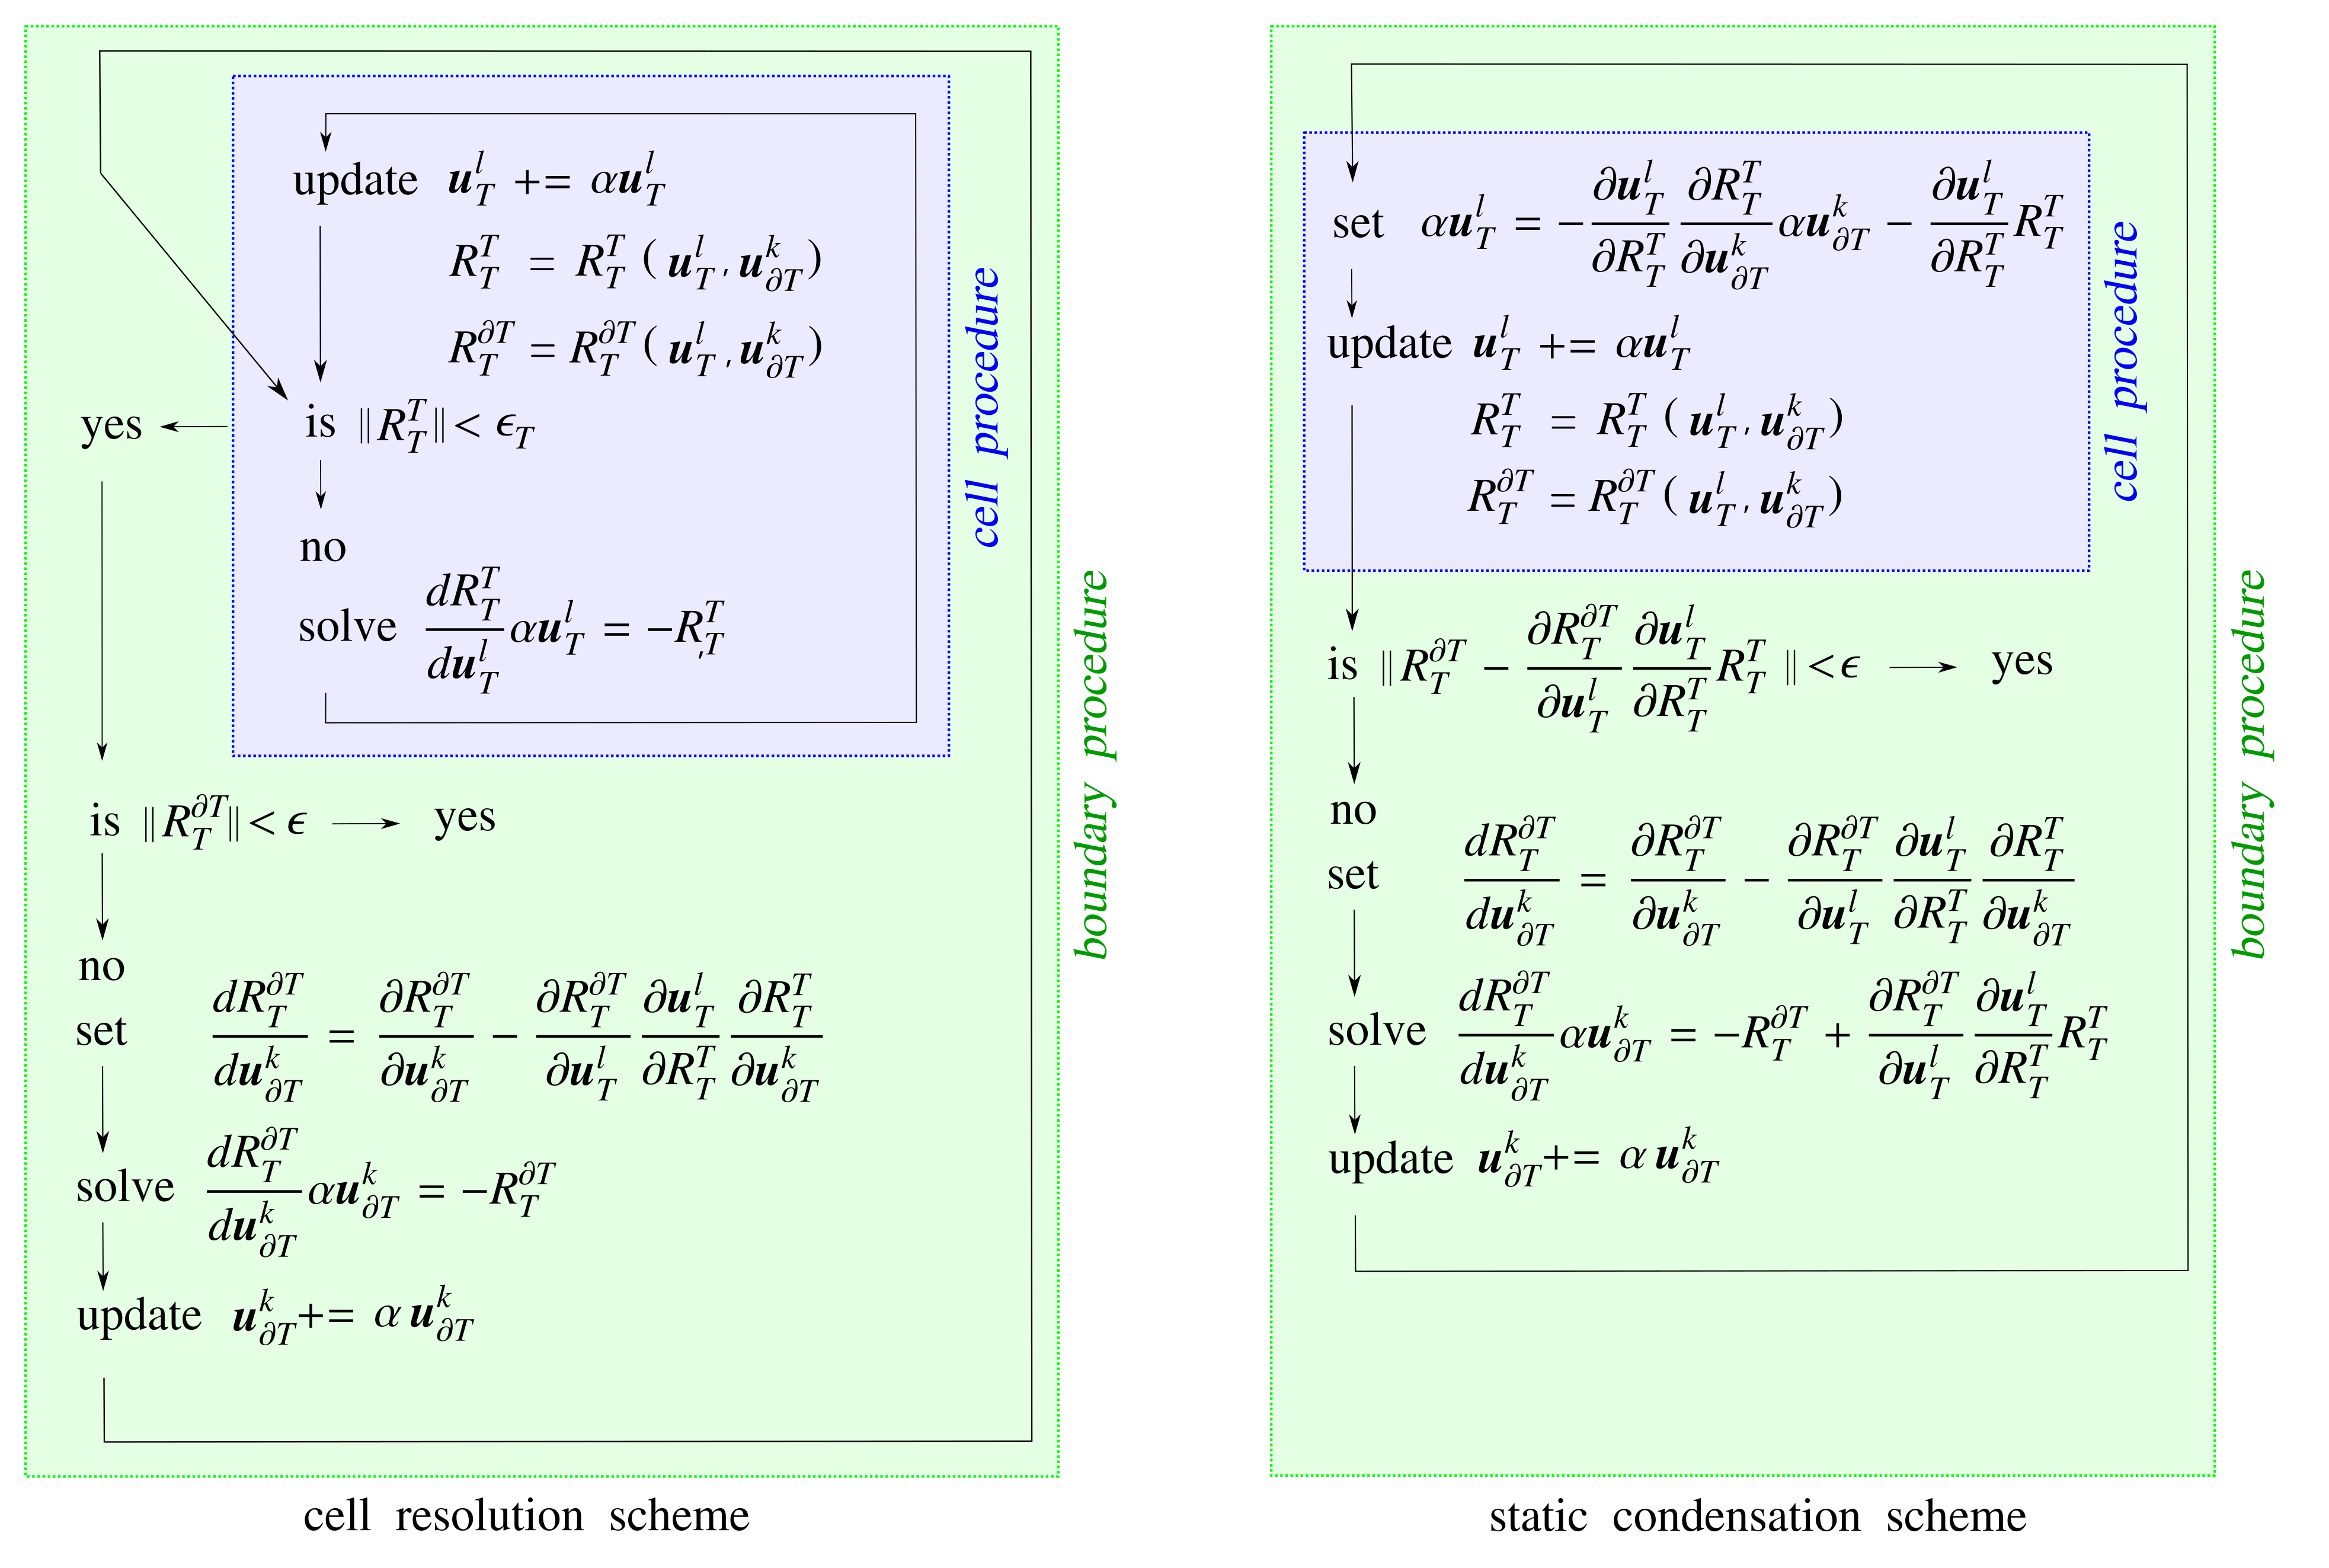
\includegraphics[width=15.cm]{img_calcs/resolution.png}
    \caption{Schematic representation of both resolution schemes}
    \label{fig_resolution}
\end{figure}

